
 % -*- coding: utf-8 -*-
%\documentclass[english]{ipsj}
%\documentclass[english,preprint]{ipsj}
\documentclass[english,preprint,JIP,technote]{ipsj}

\usepackage{graphicx}
\usepackage{latexsym}

\def\Underline{\setbox0\hbox\bgroup\let\\\endUnderline}
\def\endUnderline{\vphantom{y}\egroup\smash{\underline{\box0}}\\}
\def\|{\verb|}|

% \setcounter{volume}{26}% vol25=2017
% \setcounter{number}{1}%
% \setcounter{page}{1}


% \received{2016}{3}{4}
%\rereceived{2011}{10}{1}   % optional
%\rerereceived{2011}{10}{31} % optional
% \accepted{2016}{8}{1}


\usepackage[varg]{txfonts}%%!!
\usepackage{url}

\makeatletter%
\input{ot1txtt.fd}
\makeatother%

\begin{document}

\title{Magnet or Sticky? A Stack Overflow Tag-by-Tag Typology\\}

% \affiliate{IPSJ}{Information Processing Society of Japan, 
% Chiyoda, Tokyo 101--0062, Japan}
% \affiliate{JU}{Johoshori University, Chiyoda, Tokyo 101--0062, Japan}
% \paffiliate{PJU}{Johoshori University}
\affiliate{JU}{Graduate School of Information Science and Electrical Engineering, Kyushu University}
\affiliate{IPSJ}{Faculty of Information Science and Electrical Engineering, Kyushu University}

\author{Kotori Hieda}{JU}[hieda@f.ait.kyushu-u.ac.jp]
\author{Yu Mingzhe}{JU}[yumingzhe@f.ait.kyushu-u.ac.jp]
\author{Yasutaka Kamei}{IPSJ}[kamei@ait.kyushu-u.ac.jp]

\begin{abstract}
Stack Overflow (SO) is one of the most popular question and answer sites for software developers. SO stores posts assigned with tags that correspond to the keywords of each question. If a developer asks question related to Python and inputs ``Python'' tag on the post, the developers interested in Python can participate in the post easily. Since 2008, SO has become one of the most trusted online communities. In this study, we explore developers' interest by analyzing how they use tags. We classify tags into four: (1) attractive, (2) stagnant, (3) fluctuating, and (4) terminal based on magnet values and sticky values. We analyze data of table ``Posts'' of approximately 42 million posts in SO and table ``Users'' of approximately 9 million rows of user information. Results reveal that some historical events in IT are retrieved, which include launching of new tools and terminating of services with the transition of magnet value and sticky value.
\end{abstract}



\begin{keyword}
magnet, sticky, tag, user migration, OSS census
\end{keyword}


\maketitle

%1
\section{Introduction}
The Pew Research Center (PRC)~\cite{communityeconomic} is the U.S. fact finder that provides information on social problems and demographic trends that shape the United States and the world. \emph{Magnet states} are defined as states where a high percentage of the population migrated from the outside, whereas sticky states have a high proportion of those living in the same state since birth. Nevada is a \emph{magnet states} because  86\% of the population migrated from other states. It is possible to find the movement of American citizens by studying this demographic trend.

For software developers, understanding other developers' interests are important as the popurality of developers have advantages. Many developers like to work with convenient and easy-to-use tools. To develop a project efficiently, developers must focus on long-term-projects. 

In this study, we focus on new and existing topics of Stack Overflow (SO). Inspired by previous studies~\cite{yamashita2016magnet}, we apply Magnet and Sticky metrics to the topics collected in SO. 
The magnet metric is the number of new developers attracted to a topic and Sticky metric is the number of existing developers who stay with the topic. 
We examined the values of tags ``magnets'' and tags ``sticky'' by classifying them to the tags \emph{programming language}, \emph{framework}, and \emph{environment}. We also compared the news and history of software  companies and web services. If changes in their characteristics are discovered, we examine factors responsible for the changes based on their magnet values and sticky values. 

We address the following two research questions:

\noindent \textbf{(RQ1) What are the values of magnet and sticky in SO?}\par
In many cases, the sticky value is higher than the magnet value. In addition, the magnet value rate decreases more than that of the sticky value.

\noindent \textbf{(RQ2) How do magnet and sticky values change over time?}\par
When the status of tags moves to quadrant, we find that interesting events happen in the related tags.

\section{Definition of Magnet and Sticky} \label{magnet}
This section describes how we measure the appeal and adhesion of users on different topics. Following the Pew Research Center (PRC) definition, we use the Magnet and Sticky metrics to illustrate the migratory trends of the U.S. citizens. The PRC defines magnet states as states where a large proportion of adults are from other states. From the magnet metric, the proportion of adults residing in the magnet states were not born in the state. PRC defines the sticky state as the state where a large proportion of adults born there continue to live in the state. Thus, the sticky metric for the state is the proportion of adult residents born in the state. These definitions are good for a population study where a single adult can only occupy one state at a time. However, the definition is inapplicable to the topics discussed by the SO users as users can ask or answer questions on several topics at the same time. Therefore, we expand new definitions for SO topics.


\subsection*{\textit{\textbf{Magnet and Sticky in SO}}}

SO contents are questions and answers to the questions and comments~\cite{liu2018mining} called Posts in the  SOTorrent\cite{baltes2018sotorrent} database. Each question has one or more tags that separate the question into different topics. Posts on a question have their creator (for the question content, one is the questioner, and for the answer, one is the respondent), a participant of the topics, and the question. We also define the asking or answering questions activity on some topic as a discussion topic. For example, a classical question in SO has three tags like Java, Apache, and Linux asked by a user A and answered by a user B and C. Thus, C are participants of Java, Apache, and Linux-topics.

\noindent
\textbf{Magnet.} Magnet topics attract a large proportion of new users; thus, we calculate the magnetism of a topic as the proportion of users who ask or answer questions during the time period under new registered users in a specific year.

\noindent
\textbf{Sticky.} In sticky topics, a large proportion of the users keep participating in the discussion in the time period. Thus, we calculate the stickiness of a topic as the proportion of the users who discuss the topic in the time period.

\noindent
\textbf{Example (Calculating magnet and sticky values).}
To calculate magnet and sticky values of topics that belong to a major category, we use a total of six questions (a, b, c, d, e, f) and seven users (A, B, C, D, E, F, G); the Last Activity Date of question a, b, c was in 2017, and question d, e, f in 2018. The registration date of user A, B, C, D was in 2017, and the registration date of user E, F, G was in 2018~\cite{yamashita2016magnet}  as shown in Figure ~\ref{fig:example2}.

\begin{figure}[t]
 \centering
 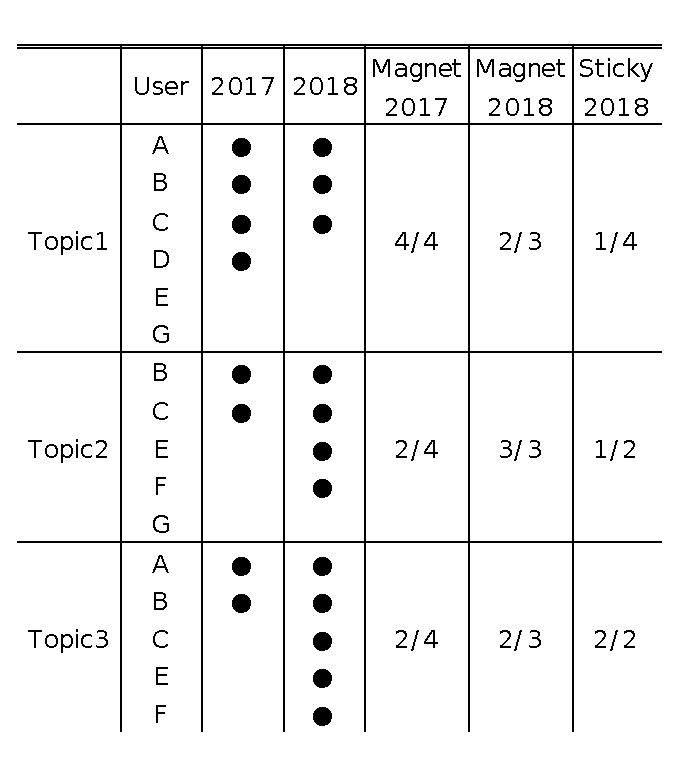
\includegraphics[width=.75\hsize]{img/explainofMS.eps}  
 \caption{Example of Magnet and Sticky values definition} 
 \label{fig:example2} 
\end{figure}


To calculate the magnet metric, we observe four new users who registered their accounts in 2017 (A, B, C, and D), and all of them discuss topic 1, whereas two of them (B, C) participate in the discussion topic 2 and 3. In this case, the Magnet value of topic 1 in 2017 is 4/4, topic 2 is 2/4, and topic 3 is 2/4.

To calculate the sticky metric on topic 1, three users participated in the discussion in 2017 (A, B, and C). Only one of them participated in the discussion in 2018 (A). Hence, the sticky value of project 1 is 1/4. In topic 2, two users participated in the discussion in 2017 (B and C); however, only one of them participated in the discussion in 2018 (B). Though new users E, F, G, participated in the discussion in 2018, we still calculate the value of sticky as 1/2. For the same reason, the sticky of topic 3 is 2/2 in 2018.\\

\noindent
\textbf{Example (Merging similar subjects into one topic).}
We merge subjects (i.e., tags) that belong to analogous subjects into one topic. For example, we consider that different version numbers (e.g., tag ``Python-2.7'' and tag ``Python-3.6'') are one of the common examples of analogous tags. 

\begin{figure}[t]
 \centering
 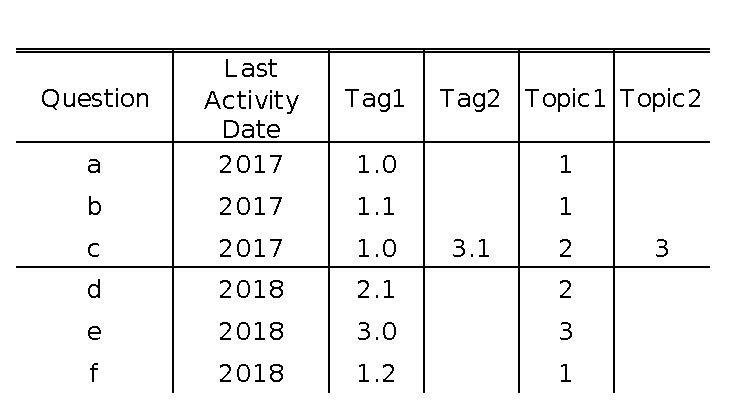
\includegraphics[width=0.80\hsize]{img/example001.eps}  
 \caption{Example of the merge of tags belonging to analogous subjects} 
 \label{fig:example1} 
\end{figure}


We also need to merge derivatives of the same technology on different platforms, merge derivatives of special tools in a certain tool family, or a combination of technology with a common used library, etc. For example, the tag ``reactjs,'' ``react-router,'' ``reactjs-flux,'' ``create-react-app'' should be merged into one topic ``react.''
% Of course, the difference in version number is the most common example of analogous tags. The rest of examples includes derivatives of the technology on different platforms, commonly used libraries, or specific tools in a tool family, etc. for example topic ``react'' includes tag ``reactjs'', ``react-router'', ``reactjs-flux'', ``create-react-app'' etc. 
We can get this information from the ``Related Tag'' column of the ``Tag Info of SO.''

Figure~\ref{fig:example1} shows that question a has tag 1.0, question b has tag 1.1, and question f has tag 1.2. According to our merge rule, they all belong to topic 1. The question c has tag 2.0 and tag 3.1, showing that it belongs to topic 2 and 3. Therefore, question d belongs to topic 2, and question e belongs to topic 3.


\begin{figure*}[t]
 \centering
 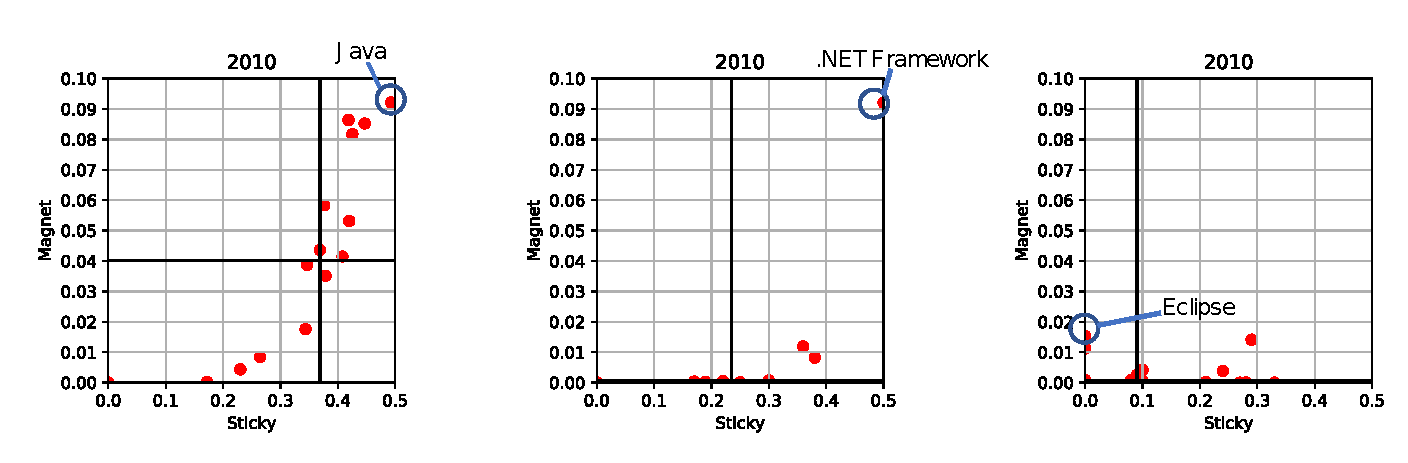
\includegraphics[width=1.0\hsize]{img/2010all.eps}  
 \caption{Distribution of Magnet and Sticky values in Programing Language, Framework and Environment} 
 \label{fig:2010} 
\end{figure*}


\section{Dataset}
We analyze the SO dataset (SOTorrent) provided by Sebastian Baltes et al.~\cite{msr2019challenge}. SOTorrent is an open dataset based on the official SO data dump and provides access to the version history of SO content at the level of whole posts and individual text or code blocks.

The dataset consists of 20 different tables stored in data on official SO data dump and data extracted from the original official SO data dump.

However, we only analyze the data from table \emph{Posts} of approximately 42 million posts from SO and table \emph{Users} of approximately 9 million rows of user information from July 2008 to September 2018. We focus on  users, tags, and time of questions. Moreover, we consider users who ask or answer questions in SO. Those who comment or like/dislike questions or answers are excluded from the statistics.

\begin{table}[t]
 \centering
 \caption{Average Quadrant Transition rate}
 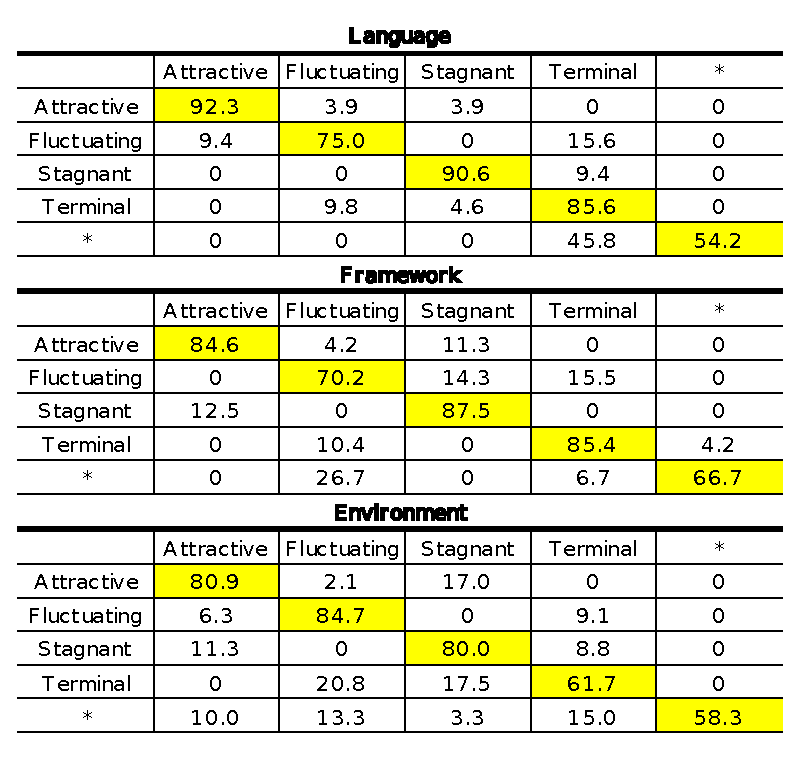
\includegraphics[width=1.0\hsize]{img/averageAFST.eps} 
 \label{table2} 
\end{table}


\section{Study Results} %paragraph4
In this section, we provide answers to these questions:
\subsection{(RQ1) What are the values of magnet and sticky in SO?}

\noindent
\textbf{Approach.}
We calculated magnet and sticky values as defined in Section~\ref{magnet}. We plot the magnet value on the vertical axis and the sticky value on the horizontal axis. We classify the plotted points into four quadrants.\\
\textbf
{Attractive:} Tags with a high magnet and sticky value. By understanding the tags, we can discover the interests of developers.\\
\textbf{Fluctuating:} Tags with a higher magnet and lower sticky value. This tag attracts people, but it is short-term. Excellent developers will be disinterested.\\
\textbf{Stagnant:} Tags with a lower magnet and higher sticky value. These tags are difficult to attract new users, but it can maintain existing users.\\
\textbf{Terminal:} Tags with the lower magnet and lower sticky value. This tag can neither attract new developers nor keep them interested.

The median of the magnet and sticky values for each year is used for the quadrant threshold because the median is unaffected by outliers. From the sticky value definition in Section~\ref{magnet}, the sticky value depends on the number of tag users in a year and the following year. To answer RQ1, we got 9 years’ worth of sticky values based on the information on the number of tag users from 2009 to 2018. The sticky value must depend on the number of new tag users, but, if the number of new tag users in a year is too low, the sticky value will be too small. To remove noise, we fix thresholds for each topic when the magnet and sticky value is less than the threshold value, it is set to 0.


We did not analyze all the tags at once, but divided them into three categories for analysis. The selected categories and their contents are:
\begin{itemize}
\item programming languages ​​(assembly, Bash, C, C♯, C ++, CSS, Go, HTML, Java, JavaScript, PHP, Python, Ruby, SQL, Swift, TypeScript)
\item frameworks ( .NET Framework, Angular, Cordova, Django, Hadoop, Node.js, React, Spark, Spring, TensorFlow, Torch, Xamarin)
\item environment (Android Studio, Atom Editor, Eclipse, Emacs, IntelliJ, IPython, Jupyter, NetBeans, Notepad++, PhpStorm, PyCharm, RStudio, RubyMine, Sublime Text, TextMate, Vim, Visual Studio, Visual Studio Code, Xcode)
\end{itemize}

We chose these tags based on SO's survey of over 100,000 developers in 2018~\footnote{\url{https://insights.stackoverflow.com/survey/2018}}. We focused on tags used by more than 5\% of developers who answered the questionnaire. 

%The year when StackOverflow released these data is May 2008. Since the sticky value is calculated from the difference between the previous year and the current year, the distribution chart of magnet and sticky value according to three categories in 2010 is shown as the first year for which yearly data of sticky value can be obtained.

% 我々は全てのタグを一度に調査するのではなく3つのカテゴリに分けて分析をした。その方が特徴を見つけやすいからである。我々が選んだカテゴリたちとその内容はプログラミング言語(assembly, Bash, C, C♯, C++, CSS, Go, HTML, Java, JavaScript, PHP, Python, Ruby, SQL, Swift, TypeScript), フレームワーク(.NET Framework, Angular, Cordova, Django, Hadoop, Node.js, React, Spark, Spring, TensorFlow, Torch, Xamarin),そして環境(Android Studio, Atom Editor, Eclipse, Emacs, IntelliJ, IPython, Jupyter, NetBeans, Notepad++, PhpStorm, PyCharm, RStudio, RubyMine, Sublime Text, TextMate, Vim, Visual Studio, Visual Studio Code, Xcode)である。
% これらを選んだ理由は2018年にStack Overflowが10万人を超える開発者たちにとったアンケートの結果に基づいている。Stack Overflowは開発者たちに使用するタグたちについてのアンケートをとり、我々はアンケートに答えた開発者たちの5\%以上が使用しているタグたちに絞って調査した。StackOverflowがこれらのデータを公開した年は2008年5月である。sticky値は前年と当年の差から算出しているため、sticky valueの通年データが取れる最初の年として2010年の3カテゴリ別のmagnetとsticky valueの分布図を示す。

% The categories we selected and their contents are programming languages (assembly, Bash, C, C\#, C++, CSS, Go, HTML, Java, JavaScript, PHP, Python, Ruby, SQL, Swift, TypeScript), framework (.NET, Angular, Cordova, Django, Hadoop, Node.js, React, Spark, Spring, TensorFlow, Torch, Xamarin), and the environment (Android Studio, Atom Editor, Eclipse, Emacs, IntelliJ, IPython, Jupyter, NetBeans, Notepad++, PhpStorm, PyCharm, RStudio, RubyMine, Sublime Text, TextMate, Vim, Visual Studio, Visual Studio Code, Xcode) because these three categories are one of the most popular tag categories used in stack overflow. We also analyzed by picking the top tags that are popular among each category. Tags that are not popular have no character and we do not know anything from that. By dividing it for each category, it became easier to see the features. We show distribution map of magnet and sticky value by 3 categories of 2010 as one of the characteristics easy to understand.

%\textbf{Manual analysis:}
%Figure~\ref{fig:2010} shows the distribution of magnet and sticky values in programing language, framework, and environment (2010)\footnote{We choose the year 2010 because it is the first year for which yearly data of sticky value can be obtained.}. 
% We find that .NET Framework is a high magnet and sticky value. 

%.NET framework 

%Beginner developers can relatively easily develop advanced software using . Are there many reasons why the .NET Framework's sticky value is high reasons most conveniently? It is the foundation system for building applications. 

%Java has long been popular and attractive as it is one of the most famous programming languages ​​in the world. Eclipse especially attracted people in 2010, so the magnet value is high.

% 図~\ref{plotframe2010}の2009 Frameworkにおいて、.NET Frameworkは高いマグネットとスティッキー値である。高いマグネットとスティッキー値であることは非常に良いと言える。.NET Framework は、2006年11月にマイクロソフトに発表された。これはネットワーク上でアプリケーションを構築する基盤のシステムである。.NET Frameworkのmagnet valueが高い理由は、初心者エンジニアでもある程度高度なソフトウェアを開発できるからである。.NET Frameworkのsticky valueが高い理由はその利便性から長く使う人が多いからだ。
% 2009 Languageにおいて、C♯のmagnet valueとsticky valueは最も高い。これは.NET構想において、C♯が中心的な開発言語であり、そのフレームワークは.NET Frameworkであることが理由のように思われる。
% 2009 Environmentにおいて、Visual Studioが高いmagnet valueとsticky valueである。Visual Studioは.NET構想を作ったMicrosoftが作った最も代表的な開発環境である。PhpStormは高いsticky valueと低いmagnet valueである。PhpStormはPHPでの開発に向いており、それはコード補完の点で優れている。PHPで開発をしない人々にとってはあまり魅力的ではないが、PHPを使う人々にとっては非常に魅力的であるためこのような結果になったと思われる。
% \medskip

\noindent \textbf{Results:}
Figure~\ref{fig:2010} shows a quadrant plot of the magnet and sticky values ​​of the 2010 framework, programming language, and environmental tag\footnote{We choose the year 2010 because it is the first year for which yearly data of sticky value can be obtained.}, revealing that the magnet value is lower than the sticky value. The results are similar to the findings of the PRC. For example, the U.S. citizens are likely to live in the same house than to change houses; it is easier for developers to continue developing the same content.
 

\noindent \textbf{Summary.}
 Tags with high magnet value are easy to use even for beginners. A tag familiar to C# has a high magnet value and sticky value, and it is more attractive.

\begin{table*}[t]
 \centering
 \caption{Quadrant Transition of Framework 2010 - 2018} 
 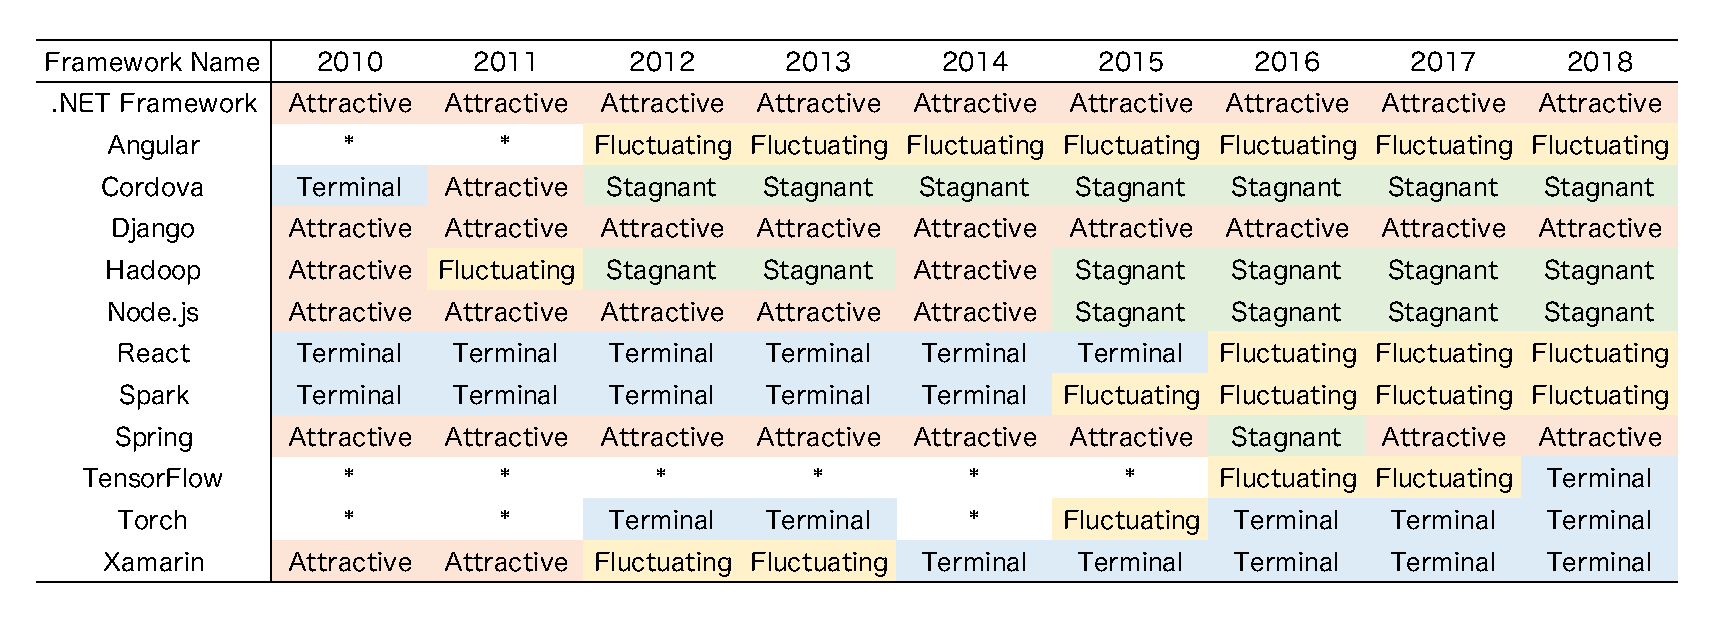
\includegraphics[width=1.0\hsize]{img/frame2010-2018.eps} 
 \label{table1} 
\end{table*}

\subsection{(RQ2) How do magnet and sticky values change over time?} 

\noindent \textbf{Approach:}
From 2010 to 2018, we calculated the probability of the tags moves quadrants from one year to the following year. For example, there were six Attractive tags in 2010. Of the six Attractive tags in 2010, five were Attractive the following year. Therefore, the transition probability from Attractive to Attractive for 2010 - 2011 is 5/6 or 83.3\%. 

\noindent \textbf{Quantitative results:}
Table~\ref{table2} shows that the proportion of the vertical axis is in the quadrant for 2010 - 2018, the horizontal axis is the year old. From the table, the ratio of tags is the highest for those that do not move the quadrants from the previous year to the following year in any programming language, framework, and environment. Since the tags have hardly changed from any quadrant to 2, once the tags have become popular to a certain extent, the users of the tags have not significantly reduced. This shows that once tags have become less popular, it may continue to be unpopular.

\noindent \textbf{Manual analysis:}
Table~\ref{table1} shows the transition of each tag quadrant in the framework, revealing how the tags move in the quadrant. Xamarin is an interesting example. Xamarin~\cite{reynolds2014xamarin} is an API for Android and iOS developed with C\#. Thus, it is difficult to develop an application without having knowledge of both applications. Developing Android and iOS apps in Windows and Visual Studio requires a lot of programming knowledge and is not good for beginners. When Xamarin was launched, it attracted the attention of many developers owing to its efficiency. However, when beginners ask questions on sites such as SO, its popularity gradually declines owing to its application difficulty for beginners.

Similarly, React~\cite{staff2016react} is a Facebook JavaScript library that builds the web application user interface efficiently. React was first launched on Facebook’s news feed in 2011 and on Instagram in 2012. It was an open source at the JSConf US on May 2013. Social networking services (SNSs)~\cite{ellison2013sociality} such as Facebook and Twitter became popular around 2015 – 2016 when React changed from Terminal to Fluctuating. Therefore, it seems that the popularity of the Framework changed based on its application on the popular SNSs.


\noindent \textbf{Summary:}
If tags were the popular tool, their popularity would decline if they were difficult to use. Even if they were not a popular tool and they turn out to be an efficient tool, they will be popular among developers.

% \begin{oframed}
%\emph{Table~\ref{table1} shows that even if it was a tool that was initially popular, its popularity would decline if it was difficult to use. Even if it was a tool that was not as popular as it was born, It turns out that as the content using the tool becomes popular, the tool also becomes popular. Table~\ref{table2} shows that it is difficult for tags to make large changes in quadrants.}
% 表1から、タグたちは四分円を大きく変遷しづらいことがわかった。また表2から、たとえ当初人気があったツールだとしても、それが使いにくいあるいは使用するのが難しいものであればその人気は減少し、また誕生当初はそこまで人気がないツールだとしても、そのツールを使用しているコンテンツが人気になればそれに伴いそのツールも人気になることがわかった。

% As a result of investigating from 2009 to 2018, in the programming language, the average transition from Attractive to Attractive was 91.5\%, the transition from Fluctuating to Fluctuating was 77.8\%, the change from Stagnant to Stagnant was 80.6\%, and the change from Terminal to Terminal was 87.2\%.  Regardless of the kind of tag, it turned out that the classification of tags was difficult to change.
% \end{oframed}


\section{Conclusions}
Critical development of a programming language, a program framework, or an operating system depends on their ability to keep the community alive and attract more people to participate in discussions. SO, the world’s largest program Q\&A platform, has enough questions and answers on a topic to solve users’ problems. This study applied the magnet and sticky population concepts to explore topics in SO. The results show that the numbers of participating topics are exploding with the development of computer technology. Even the most popular themes that did not attract people’s attention 10 years ago now attract a large number of participants. Under respective major categories, the most popular topics are still very popular after 10 years, and only a small number of languages or frameworks can become one of the most popular topics. This research provides a reference for enterprises to choose their main technology stack. It can also be used as a reference for computer science students to learn new technologies. The study (1) can predict the trend of computer technology in the next few years and (2) can identify easier technologies to access the questions and answers.

% 1. The number of topics that people participate in is exploding with the development and popularity of computer technology. Even the most popular themes cannot attract the high percentage of people involved in the discussion like swhat they did ten years ago.
% \smallskip\smallskip

% 2. Under their respective major categories, the most popular topics are still very popular after ten years, and only a small number of languages or frameworks can stand out and become one of the most popular topics.
% \smallskip\smallskip

% 3. This research can provide some reference for enterprises to choose their own main technology stack, and can also be used as a reference for computer science students to learn new technologies, because it (1) predicts the trend of computer technology in the next few years, (2) points out which technologies are easier to access and the questions can be easier to get answers to.

\bibliographystyle{IEEEtran}
\bibliography{mining}

\end{document}
